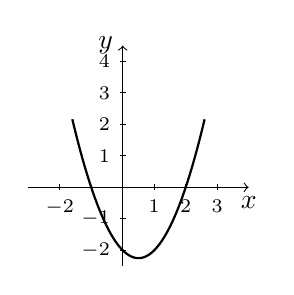
\begin{tikzpicture}[scale=0.4]
    \draw[->] (-3,0) -- (4,0) node[below] {$x$};
    \draw[->] (0,-2.5) -- (0,4.5) node[left] {$y$};

    \foreach \x in {-2,1,2,3}
        \draw (\x,0.1) -- (\x,-0.1) node[below] {\scriptsize $\x$};

    \foreach \y in {-2,-1,1,2,3,4}
        \draw (0.1,\y) -- (-0.1,\y) node[left] {\scriptsize $\y$};

    % y = x^2 - x - 2 = (x+1)(x-2)
    \draw[smooth, samples=200, domain=-1.6:2.6, thick]
        plot (\x, {\x*\x - \x - 2});

    \fill (-1,0) circle (1.5pt);
    \fill (2,0) circle (1.5pt);
\end{tikzpicture}